% !TEX program = xelatex
% Cards format — auto-generated from kidlisp.tex by cards-convert.mjs
\documentclass[11pt]{article}

\usepackage{fontspec}
\usepackage{unicode-math}
\setmainfont{Latin Modern Roman}
\setsansfont{Latin Modern Sans}
\setmonofont{Latin Modern Mono}[Scale=0.88]


\usepackage{graphicx}
\graphicspath{{figures/}}
\usepackage{booktabs}
\usepackage{tabularx}
\usepackage{ragged2e}
\usepackage{microtype}
\usepackage{natbib}
\usepackage{listings}

\newfontfamily\kidlispbold{ywft-processing-bold}[
  Path=../../system/public/type/webfonts/,
  Extension=.ttf
]
\newfontfamily\kidlispfont{ywft-processing-light}[
  Path=../../system/public/type/webfonts/,
  Extension=.ttf
]

\makeatletter
\def\input@path{{../}}
\makeatother
\usepackage{ac-paper-cards}

\hypersetup{
  pdftitle={KidLisp '26: A Minimal Lisp for Generative Art},
}

\begin{document}

% ============================================================
% TITLE CARD
% ============================================================
\thispagestyle{empty}
\vspace*{\fill}
\begin{center}

\includegraphics[height=3em]{pals}\par\vspace{0.6em}
{\acbold\fontsize{20pt}{24pt}\selectfont\color{acdark} Kid{\color{acpurple}Lisp} '26}\par
\vspace{0.3em}
\vspace{0.5em}
{\normalsize Jeffrey Alan Scudder}\par
{\small\color{acgray} Aesthetic Inc.}\par
{\small\color{acgray} ORCID: \href{https://orcid.org/0009-0007-4460-4913}{0009-0007-4460-4913}}\par
\vspace{0.8em}
\rule{0.6\textwidth}{1pt}\par
\vspace{0.4em}
{\small\color{acpink}\textbf{[ working draft --- not for citation ]}}\par
\vspace{0.3em}
{\footnotesize\color{acgray} March 2026}\par
\end{center}
\vspace*{\fill}

% ============================================================
% BODY
% ============================================================
\section{Introduction}

Creative coding environments typically require users to learn a general-purpose programming language before producing visual or sonic output. Processing~\citep{reas2007processing} uses Java; p5.js~\citep{mccarthy2015p5js} uses JavaScript; Sonic Pi~\citep{aaron2016sonic} uses Ruby-like constructs. While these tools have dramatically lowered the barrier to computational expression, they still demand familiarity with variables, functions, control flow, and---in many cases---a local development environment.

\kidlisp{} starts from a different question: \emph{what is the smallest language that can produce interesting generative art?} The answer is a Lisp with carefully chosen built-in functions, no user-defined procedures, and a browser-native runtime requiring no installation. A complete animated program can be a single line:

\begin{lstlisting}
(ink |\kt{rainbow}|) (repeat |\kn{100}| |\kv{i}|
  (circle (wiggle width) (wiggle height) |\kn{10}|))
\end{lstlisting}

The design is motivated by observations from No Paint~(2020), a pixel art tool whose community of non-technical users demonstrated that people learn computing through social participation in software they love. \kidlisp{} extends this insight into a programming language: every program is immediately shareable by a short code, viewable at a URL, and embeddable inside other programs.

This paper describes the language design~(\S\ref{sec:design}), evaluator architecture~(\S\ref{sec:architecture}), the storage and distribution infrastructure~(\S\ref{sec:infrastructure}), media pipeline~(\S\ref{sec:media}), and adoption data~(\S\ref{sec:evaluation}).

\begin{figure}[t]
\centering
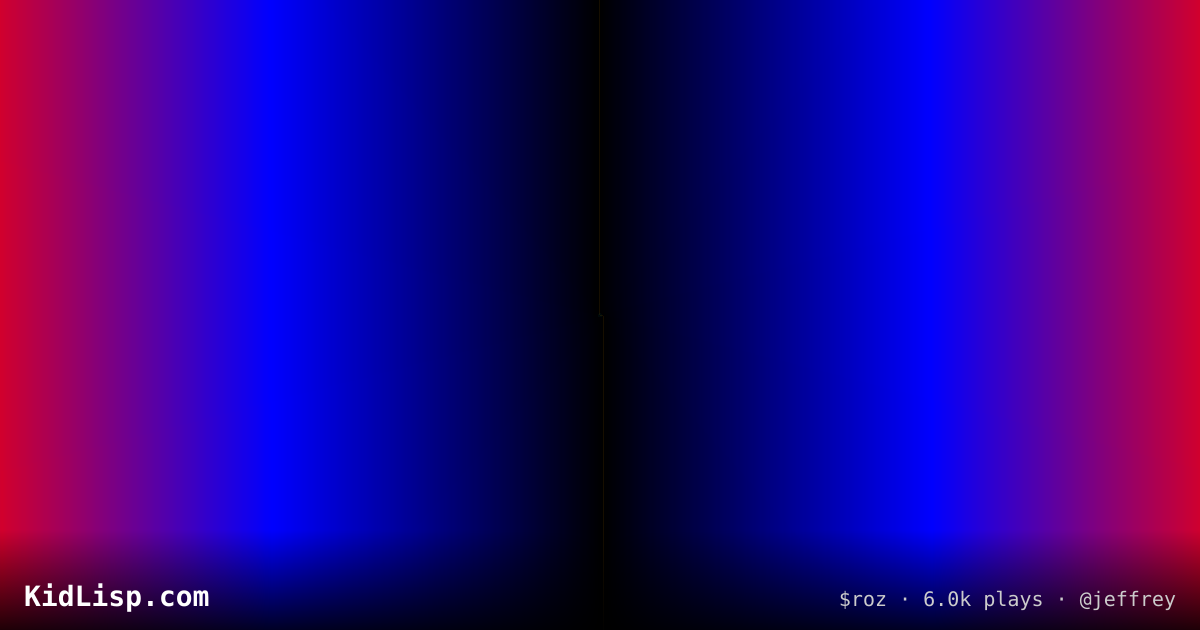
\includegraphics[width=\columnwidth]{kidlisp-og-mosaic.png}
\caption{A featured \kidlisp{} program (\texttt{\$roz}) as rendered by the oven service for Open Graph social previews. The overlay shows the program code, play count, and author handle.}
\label{fig:og}
\end{figure}

% ============ 2. LANGUAGE DESIGN ============

\section{Language Design}
\label{sec:design}

\kidlisp{} is an S-expression language. Every program is a sequence of expressions evaluated top-to-bottom, producing side effects on an HTML Canvas 2D context, a WebGL context, a Web Audio graph, or some combination thereof.

\subsection{Design Principles}

\begin{enumerate}
  \item \textbf{Every expression draws.} Valid \kidlisp{} produces visible output. There is no \texttt{main}, no imports, no boilerplate.
  \item \textbf{Flat over deep.} Programs are composed by embedding other programs, not by defining abstractions. This keeps code readable at a glance.
  \item \textbf{Safe by construction.} No file I/O, no networking, no mutation of external state. Programs are sandboxed by the language's lack of dangerous primitives.
  \item \textbf{Social by default.} Every program gets a short code and a URL. Sharing is the distribution mechanism, not an afterthought.
\end{enumerate}

\subsection{Function Categories}

The 118 built-in functions span 12 categories (Table~\ref{tab:functions}).

\begin{table}[h]
\small
\centering
\begin{tabularx}{\columnwidth}{lrX}
\toprule
\textbf{Category} & \textbf{n} & \textbf{Examples} \\
\midrule
Graphics & 9 & \texttt{wipe}, \texttt{ink}, \texttt{line}, \texttt{box}, \texttt{circle} \\
Transforms & 11 & \texttt{scroll}, \texttt{zoom}, \texttt{spin}, \texttt{blur}, \texttt{suck} \\
Math & 14 & \texttt{+}, \texttt{sin}, \texttt{cos}, \texttt{random}, \texttt{wiggle} \\
Colors & 19 & CSS names + \texttt{rainbow}, \texttt{zebra} \\
System & 9 & \texttt{width}, \texttt{height}, \texttt{frame}, \texttt{fps} \\
3D & 8 & \texttt{cube}, \texttt{form}, \texttt{trans}, \texttt{move} \\
Audio & 6 & \texttt{mic}, \texttt{melody}, \texttt{overtone} \\
Control & 7 & \texttt{def}, \texttt{if}, \texttt{repeat}, \texttt{once}, \texttt{later} \\
Text & 4 & \texttt{write}, \texttt{type}, \texttt{paste} \\
Input & 3 & \texttt{pen}, \texttt{touch} \\
Composition & 4 & \texttt{embed}, \texttt{layer}, \texttt{fade} \\
Data & 4 & \texttt{let}, \texttt{list}, \texttt{get}, \texttt{set} \\
\midrule
\textbf{Total} & \textbf{118} & \\
\bottomrule
\end{tabularx}
\caption{Built-in functions by category.}
\label{tab:functions}
\end{table}

\begin{figure}[t]
\centering
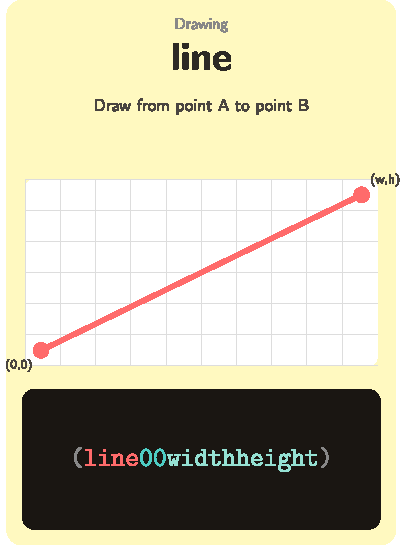
\includegraphics[height=4.5cm]{card-line.pdf}%
\hfill%
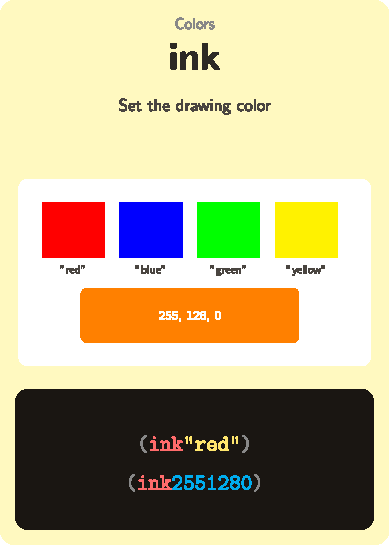
\includegraphics[height=4.5cm]{card-ink.pdf}
\caption{\kidlisp{} reference cards for the \texttt{line} and \texttt{ink} functions, showing syntax and coordinate output. Cards are distributed as SVG illustrations at \texttt{kidlisp.com/cards}.}
\label{fig:cards}
\end{figure}

\subsection{Timing Syntax}

\kidlisp{} provides temporal operators that schedule expression evaluation without explicit loops or callbacks:

\begin{lstlisting}
|\kt{2.5s}| (wipe |\kt{red}|)           ; after 2.5 seconds
|\kt{1s...}| (spin |\kn{5}|)            ; repeat every second
|\kt{3s!}| (write "Done" |\kn{10}| |\kn{10}|)  ; fire exactly once at 3s
|\kt{30f}| (ink |\kt{blue}|)             ; after 30 frames
\end{lstlisting}

The suffix \texttt{s} denotes seconds, \texttt{f} denotes frames, \texttt{...} denotes repetition, and \texttt{!} denotes one-shot execution. These operators compose: \texttt{0.5s... (ink (random 255) (random 255) (random 255))} produces a color change every half-second.

\subsection{What KidLisp Omits}

The language deliberately excludes user-defined functions (beyond \texttt{def} for named values), recursion, string manipulation, file I/O, networking, mutable data structures, and exception handling. These omissions are the design. By removing abstraction mechanisms, programs remain flat and legible---a reader can understand any program top-to-bottom without tracing call stacks.

% ============ 3. ARCHITECTURE ============

\section{Evaluator Architecture}
\label{sec:architecture}

The evaluator (\texttt{kidlisp.mjs}, 15,161 lines) is a single JavaScript ES module implementing a tree-walking interpreter.

\subsection{Evaluation Model}

The evaluator runs once per animation frame. S-expressions are tokenized and parsed into a nested array AST, then walked with dispatch on the first symbol of each list. Built-in functions map directly to Canvas 2D operations, WebGL commands, Web Audio API calls, and mathematical computations. The entire program is re-evaluated each frame, with \texttt{frame} and \texttt{time} bindings updated automatically---an immediate-mode model that eliminates explicit animation loops.

\subsection{Deterministic Rendering}

Given the same random seed and frame count, a program always produces identical output. The \texttt{random} function uses a seeded PRNG initialized from the program's short code, enabling reproducible generative art.

\subsection{Chaos Mode}

Invalid or random text input triggers artistic visual output rather than error messages. A confidence-scored detector examines word recognition rate ($<$30\% known words), special character ratio ($>$50\%), and parenthesis balance (ratio $>$3:1) to classify input as code or chaos. Chaotic input produces deterministic generative visuals seeded from the input text. This means that \emph{any} text typed into \kidlisp{} produces something visual---there are no error states visible to the user.

\subsection{Performance}

The evaluator implements three levels of optimization:

\begin{itemize}
  \item \textbf{Multi-level code cache}: Embedded program resolution checks RAM, then IndexedDB, then network, then TEIA (a decentralized archive). Cache hits avoid re-parsing and re-fetching.
  \item \textbf{Buffer pooling}: Up to 8 reusable offscreen canvases per resolution, avoiding allocation churn during compositing.
  \item \textbf{Auto-density scaling}: Pixel density adjusts between 0.5x and 4x based on a rolling FPS average (target: 30--55 FPS), with a 60-frame cooldown between adjustments.
\end{itemize}

Function call results, alpha-adjusted pixel buffers, and blend composites are individually cached and invalidated per frame.

% ============ 4. INFRASTRUCTURE ============

\section{Storage and Distribution}
\label{sec:infrastructure}

\subsection{MongoDB Storage}

Each program is stored as a document in the \texttt{kidlisp} MongoDB collection:

\begin{lstlisting}[language=json]
{
  "code": "cow",
  "source": "(wipe blue)\n(ink yellow)...",
  "hash": "a3f2e8...",
  "when": "2025-06-15T...",
  "lastAccessed": "2026-03-01T...",
  "hits": 342,
  "user": "auth0|abc123"
}
\end{lstlisting}

The \texttt{hash} field (SHA-256 of the trimmed source) enforces content-addressed deduplication: identical programs always resolve to the same code. The \texttt{hits} counter and \texttt{lastAccessed} timestamp enable usage analytics. The collection maintains unique indexes on both \texttt{code} and \texttt{hash}, plus sparse indexes on \texttt{user} and optional NFT mint records (\texttt{kept.network}).

\subsection{Code Generation}

Short codes are generated by a source-aware algorithm. The system first attempts to derive a meaningful code from the program's content---extracting dominant function names, color keywords, or structural patterns---falling back to random \texttt{nanoid} generation if all inferred codes are taken. This produces codes like \texttt{cow} (a program with cow-like shapes) rather than arbitrary alphanumeric strings.

\subsection{REST API}

The storage endpoint (\texttt{store-kidlisp.mjs}) provides five query modes over a single URL:

\begin{enumerate}
  \item \textbf{POST} --- Store a program. Deduplicates by SHA-256 hash, generates a short code, optionally syncs to ATProto (Bluesky) and publishes a profile event.
  \item \textbf{GET \texttt{?code=xyz}} --- Retrieve a single program with the author's handle resolved via \texttt{\$lookup} on the \texttt{@handles} collection.
  \item \textbf{GET \texttt{?codes=a,b,c}} --- Batch retrieval (up to 50 codes) for embedded layer resolution during evaluation.
  \item \textbf{GET \texttt{?recent=true}} --- Paginated feed sorted by creation time or hit count, with optional \texttt{handle} filter for per-user feeds.
  \item \textbf{GET \texttt{?stats=functions}} --- Function usage analytics across the corpus, returning weighted counts by program popularity.
\end{enumerate}

Authentication is optional with a 3-second timeout---anonymous program creation is supported, but authenticated users get attribution and profile event publishing.

\subsection{Embedding and Composition}

The \texttt{\$code} syntax inside a program triggers a fetch from the storage API (or cache hit), evaluation in an offscreen buffer, and compositing onto the parent canvas. This creates a directed acyclic composition graph. A real example:

\begin{lstlisting}
; A 3D grid of cubes with embedded layers
(wipe |\kt{black}|)
(def |\kv{gridsize}| |\kn{6}|)
(repeat (|\km{*}| |\kv{gridsize}| |\kv{gridsize}|) |\kv{i}|
  (ink (hop |\kn{0.1}| |\kt{rainbow}| |\kt{blue}| |\kt{white}|))
  (form (trans (cube |\kv{i}|)
    (move (|\km{*}| (|\km{\%}| |\kv{i}| |\kv{gridsize}|) |\kn{3}|) |\kn{0}| |\kn{-20}|)
    (scale |\kn{1.5}|) (spin |\kn{0}| |\kn{1}| |\kn{0}|))))
(|\ke{\$27z}|)
(|\ke{\$cow}|)
\end{lstlisting}

Here \texttt{\$27z} and \texttt{\$cow} are resolved from MongoDB, rendered into offscreen buffers, and composited. Users build complex visuals by layering simple programs rather than writing complex single programs.

% ============ 5. MEDIA PIPELINE ============

\section{Media Pipeline}
\label{sec:media}

The oven service (\texttt{oven.aesthetic.computer}) converts recorded \kidlisp{} sessions into shareable media assets.

\subsection{Recording to MP4}

When a user records a session, the session server uploads a ZIP containing PNG frames and optional WAV audio. The oven:

\begin{enumerate}
  \item Extracts frames and reads \texttt{timing.json} for per-frame durations
  \item Generates a thumbnail from the middle frame (3x nearest-neighbor upscale, fitted to 512$\times$512)
  \item Encodes to H.264/AAC MP4 via FFmpeg with nearest-neighbor upscaling to preserve pixel art aesthetics
  \item Uploads to DigitalOcean Spaces CDN
  \item Stores bake metadata in the \texttt{oven-bakes} MongoDB collection and notifies subscribers via WebSocket
\end{enumerate}

The oven watches the \texttt{tapes} MongoDB collection via a change stream, automatically detecting new recordings that need processing.

\begin{figure}[t]
\centering
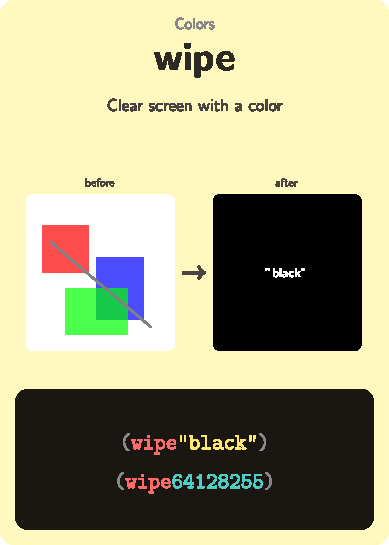
\includegraphics[height=4.5cm]{card-wipe.pdf}%
\hfill%
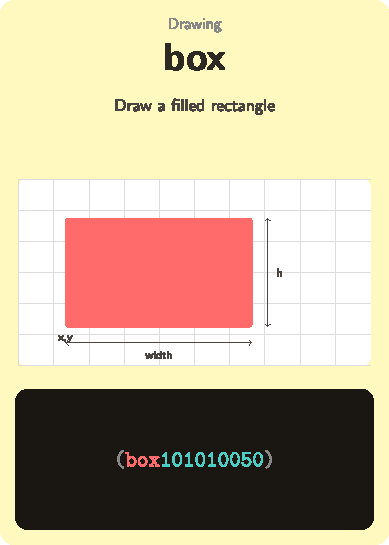
\includegraphics[height=4.5cm]{card-box.pdf}
\caption{Reference cards for \texttt{wipe} (clear screen with color) and \texttt{box} (draw rectangle). Each card shows the function signature, a visual example on a grid, and the corresponding source code.}
\label{fig:cards2}
\end{figure}

\subsection{Social Preview Images}

The oven generates Open Graph preview images for social sharing at stable URLs (e.g., \texttt{/kidlisp-og.png}). iOS crawlers require direct image serving---they will not follow 301 redirects on \texttt{og:image} URLs---so the oven caches generated PNGs and serves them with immediate 200 responses, triggering asynchronous regeneration on cache misses.

\subsection{Asset Delivery}

All media assets are served via DigitalOcean Spaces CDN (\texttt{art-aesthetic-computer.sfo3.cdn.\allowbreak digitaloceanspaces.com}). Recorded tapes use a separate bucket (\texttt{at-blobs-aesthetic-computer}) with an optional custom CDN domain. Netlify proxies \texttt{/preview/*} and \texttt{/icon/*} paths to the oven for transparent URL resolution.

% ============ 6. IDE ============

\section{Development Environment}

The \kidlisp{} IDE at \texttt{kidlisp.com} provides a Monaco-based editor with custom syntax highlighting, a live preview iframe running the Aesthetic Computer runtime, a console panel, and playback controls (play/pause/stop).

A ``slide mode'' allows dragging numeric literals in the editor to adjust values in real time---the cursor becomes a horizontal slider over any number, and the preview updates continuously during the drag.

The IDE supports two layout modes: \emph{studio} (split-pane editor, preview, and console) and \emph{stage} (editor overlaid directly on the full-screen canvas with transparent background, all chrome hidden). Stage mode is designed for live performance contexts where the code itself becomes part of the visual output.

% ============ 7. DEVELOPMENT HISTORY ============

\section{Development History}
\label{sec:history}

The following timeline is reconstructed from the git history of the Aesthetic Computer repository (626 commits touching \texttt{kidlisp.mjs} between April 2024 and March 2026).

\subsection{Phase 1: Prototype (April--June 2024)}

Development began on April 17, 2024 with a commit titled ``mock lisp.'' Within three days, the S-expression parser was working, \texttt{ink} and \texttt{line} accepted numeric parameters, and programs could be entered directly in the AC prompt. By late April, \texttt{def} was added for variable definitions. May and June 2024 saw 66 commits adding core drawing functions, the \texttt{later} timing construct, \texttt{once} for one-shot execution, and anonymous publishing of programs. The evaluator reached approximately 1,000 lines.

\subsection{Phase 2: Hiatus (July 2024--May 2025)}

No commits touched \texttt{kidlisp.mjs} for 11 months. The language existed as a working prototype embedded in the AC prompt but lacked a storage backend, embedding, audio, or a dedicated editor.

\subsection{Phase 3: Rapid Expansion (June--August 2025)}

Development resumed in June 2025 with 82 commits that month. The evaluator grew from 1,760 to 4,965 lines by August. Key additions:

\begin{itemize}
  \item \textbf{June 2025}: Melody parser, clock syntax, per-frame rendering model, test suite (\texttt{kidlisp-spec.js}).
  \item \textbf{July 2025}: MongoDB storage backend (\texttt{store-kidlisp.mjs}), short code generation, QR code sharing, tape recording and GIF export, microphone input (\texttt{mic}) with fallback animations.
  \item \textbf{August 2025}: Embedded layers (\texttt{\$code} syntax) with alpha compositing and offscreen buffering, Tezos blockchain integration for minting programs as NFTs, \texttt{fade} gradients, and pixel buffer optimizations.
\end{itemize}

The evaluator crossed 10,000 lines by late September 2025.

\subsection{Phase 4: Platform Integration (September--December 2025)}

With 108 commits in October alone (the peak month), this phase integrated \kidlisp{} into the broader Aesthetic Computer ecosystem:

\begin{itemize}
  \item \textbf{September 2025}: Layer 0 architecture (erase mode), bake layering for MP4 export, performance-critical embedded layer fixes.
  \item \textbf{October 2025}: ATProto/Bluesky federation (programs syndicated as social media posts), PACK mode for platform-agnostic bundling, slide mode for real-time numeric parameter adjustment.
  \item \textbf{November 2025}: \texttt{kidlisp.com} IDE launched (Monaco editor, live preview, console, playback controls), execution trace system for debugging, NFT workflow renamed from ``OBJKT'' to ``keep.''
  \item \textbf{December 2025}: Reference cards (SVG illustrations for each function), IPFS thumbnail generation for NFTs, oven OG image generation for social sharing, auto-density performance scaling.
\end{itemize}

\subsection{Phase 5: Refinement (January--March 2026)}

The evaluator stabilized at 15,161 lines. Additions included chaos mode (February 2026), 3D primitives (\texttt{cube}, \texttt{form}, \texttt{trans}), frequency band audio variables, the \texttt{flip} command, and stage mode for live performance. Development shifted from feature addition to robustness: fixing embedded layer performance regressions, preventing chaos mode misclassification, and improving cache invalidation.

\begin{table}[h]
\small
\centering
\begin{tabular}{lrl}
\toprule
\textbf{Date} & \textbf{Lines} & \textbf{Milestone} \\
\midrule
Apr 2024 & 0 & Initial commit (``mock lisp'') \\
Jun 2024 & $\sim$1{,}000 & Core drawing, timing, variables \\
Jun 2025 & 1{,}760 & Development resumes \\
Aug 2025 & 4{,}965 & Embedding, audio, storage \\
Sep 2025 & 10{,}382 & Layer architecture, baking \\
Dec 2025 & 13{,}877 & IDE, cards, OG images \\
Feb 2026 & 15{,}161 & Chaos mode, 3D, refinement \\
\bottomrule
\end{tabular}
\caption{Evaluator growth by line count (\texttt{kidlisp.mjs}).}
\label{tab:growth}
\end{table}

% ============ 8. EVALUATION ============

\section{Evaluation}
\label{sec:evaluation}

Adoption metrics as of March 2026 are shown in Table~\ref{tab:adoption}.

\begin{table}[h]
\small
\centering
\begin{tabular}{lr}
\toprule
\textbf{Metric} & \textbf{Value} \\
\midrule
Total programs created & 16,174 \\
Unique authors & 59 \\
Programs per author (median) & 12 \\
Programs per author (top quartile) & 180+ \\
Embedding depth (max observed) & 7 layers \\
Platform registered users & 2,798 \\
\bottomrule
\end{tabular}
\caption{Adoption metrics (March 2026).}
\label{tab:adoption}
\end{table}

\subsection{Function Usage Analytics}

The \texttt{?stats=functions} API endpoint provides weighted function usage counts across the corpus. It scans up to 5,000 programs (sorted by hits), parses each source to extract function calls, and returns counts weighted by program popularity. This enables quantitative analysis of which primitives users gravitate toward. The most-used functions are \texttt{wipe}, \texttt{ink}, \texttt{repeat}, and \texttt{circle}---confirming that users primarily engage with drawing and iteration.

\subsection{Observations}

\textbf{Composition over abstraction.} Users embed rather than abstract. The most-referenced programs are simple visual primitives (gradients, shapes, patterns) that serve as building blocks.

\textbf{Exploration over engineering.} Programs are typically short (under 10 lines). Users iterate by saving new programs rather than editing existing ones, creating divergent exploration paths visible in the storage timestamps.

\textbf{Social learning.} The most prolific authors began by viewing and remixing existing programs. The short code system makes discovery accidental---users encounter programs by trying random codes.

\subsection{Limitations}

\kidlisp{} is not suitable for general-purpose programming, complex simulations, or applications requiring state persistence across sessions. The lack of user-defined functions limits program complexity---a deliberate choice, but one that some advanced users find frustrating.

% ============ 8. RELATED WORK ============

\section{Related Work}

\textbf{Creative coding.} Processing~\citep{reas2007processing} and p5.js~\citep{mccarthy2015p5js} are the dominant tools. OpenFrameworks uses C++. All require managing a project structure and understanding a general-purpose language.

\textbf{Live coding.} Hydra~\citep{hydra2019} provides browser-based live visual coding with JavaScript method chaining but no persistent storage or social features. Sonic Pi~\citep{aaron2016sonic} targets music education. Fluxus~\citep{fluxus2007} used Scheme for 3D visuals but is no longer maintained.

\textbf{Educational languages.} Scratch~\citep{resnick2009scratch} demonstrated that social sharing drives engagement in educational programming. \kidlisp{} inherits this insight but uses text-based Lisp syntax and targets generative art rather than general education.

\textbf{Lisp for art.} Racket's \texttt{2htdp/image} library~\citep{racket2018} provides functional image construction for CS education but targets static images and pedagogy, not real-time animation with social distribution.

% ============ 9. CONCLUSION ============

\section{Conclusion}

\kidlisp{} demonstrates that a minimal domain-specific language---browser-native, no user-defined abstractions, backed by a content-addressed database with social distribution---can support a productive community of generative art practitioners. The key design insight is that social distribution (short codes, URL sharing, embedding) is not an add-on but a core language feature that shapes how users learn, create, and build on each other's work.

The embedding graph, function usage analytics API, and corpus of 16,000+ timestamped programs with author attribution constitute a dataset for studying creative coding practices, computational creativity, and how non-expert users learn functional programming through social participation.

\kidlisp{} is open source under the ISC license. The evaluator, documentation, and tools are available at \url{https://github.com/digitpain/aesthetic.computer}. Programs can be browsed and created at \url{https://kidlisp.com}.

\vspace{0.5em}
\noindent\textbf{ORCID:} \href{https://orcid.org/0009-0007-4460-4913}{0009-0007-4460-4913}

% ============ REFERENCES ============

\bibliographystyle{plainnat}
\bibliography{references}

\end{document}
